\begin{figure}[htb!]
\centering
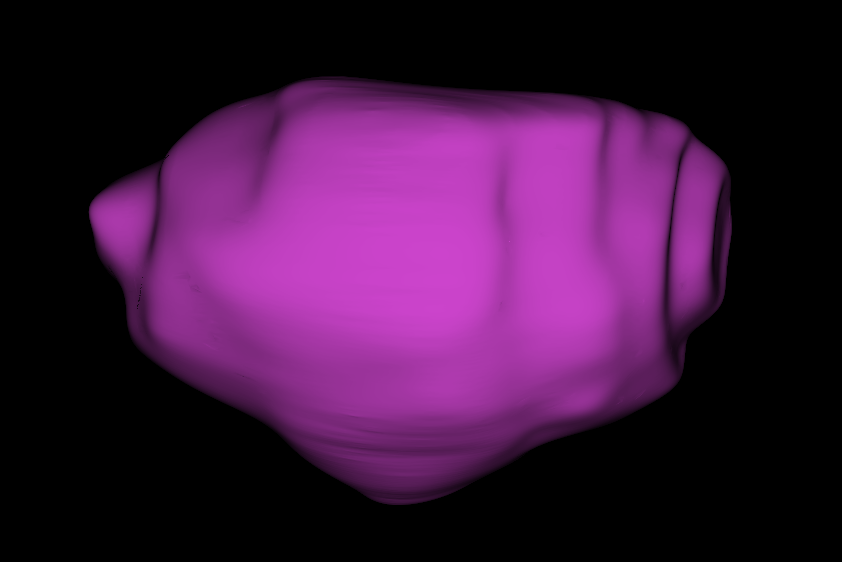
\includegraphics[width=0.3\textwidth]{tyler/3D_capsule.png} \\
Prostate Capsule \\
\vspace{3 mm}
\begin{tabular}{ccc}
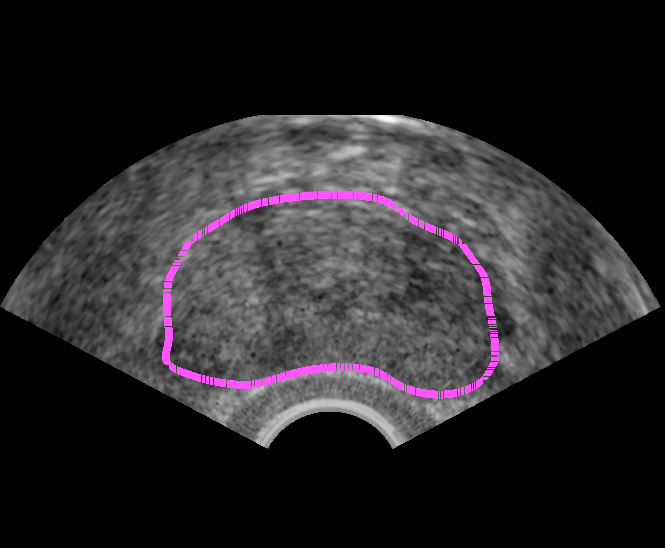
\includegraphics[width=0.3\textwidth]{tyler/axial_bmode.png} &
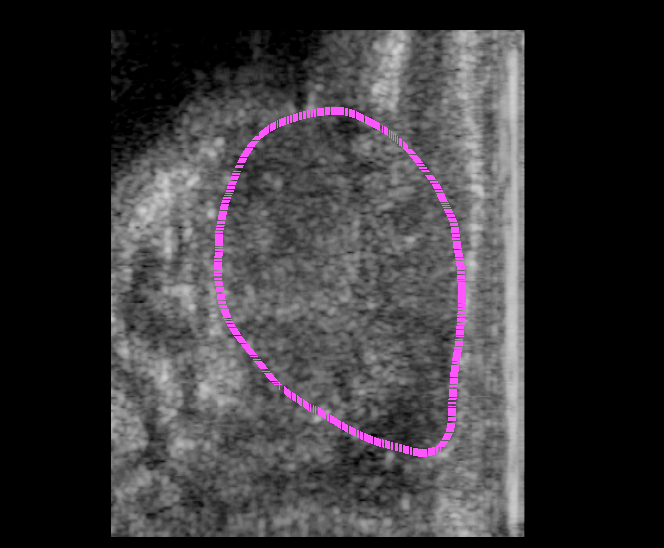
\includegraphics[width=0.3\textwidth]{tyler/sagittal_bmode.png} &
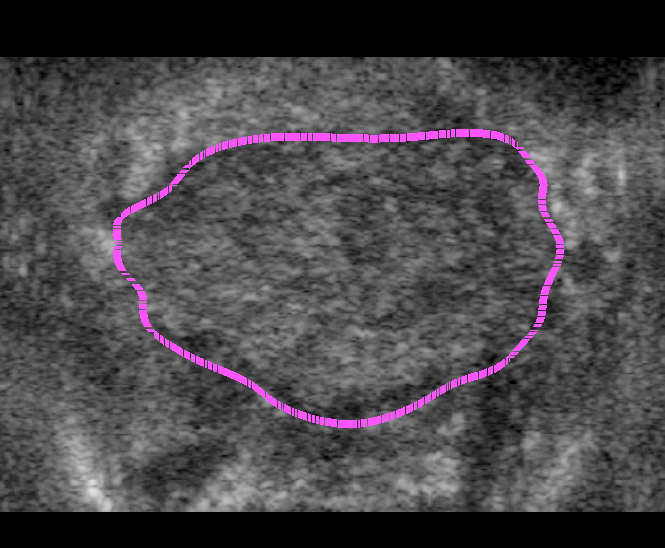
\includegraphics[width=0.3\textwidth]{tyler/coronal_bmode.png} \\
Axial B-mode Outline & Sagittal B-mode Outline & Coronal B-mode Outline \\
\vspace{5 mm}
\end{tabular}
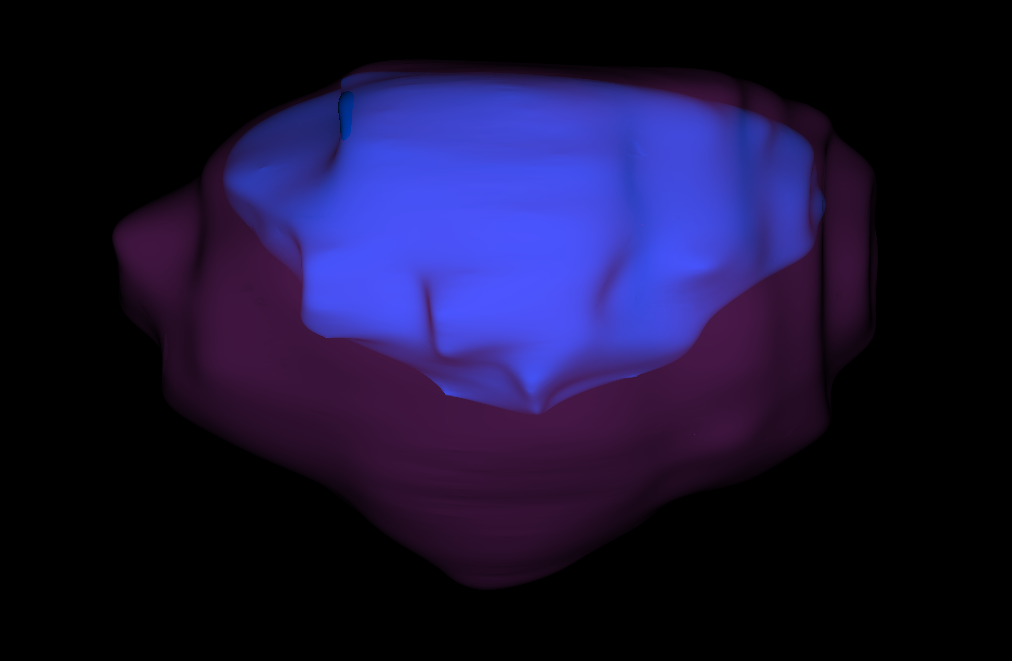
\includegraphics[width=0.3\textwidth]{tyler/3D_CG.png} \\
Prostate Central Gland \\
\vspace{3 mm}
\begin{tabular}{ccc}
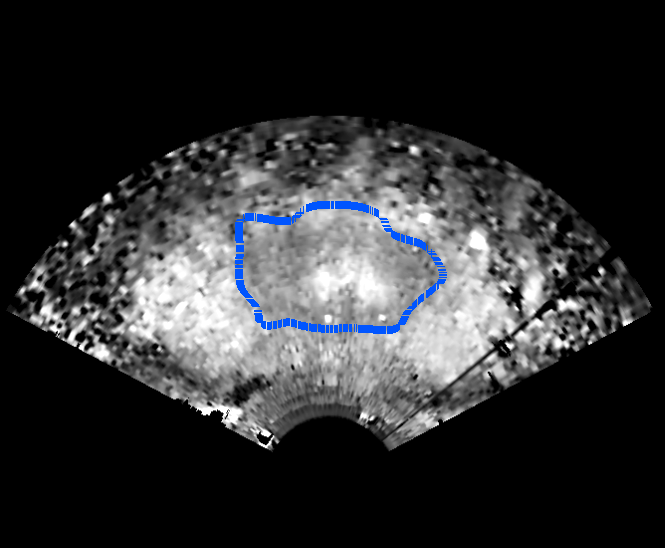
\includegraphics[width=0.3\textwidth]{tyler/axial_ARFI.png} &
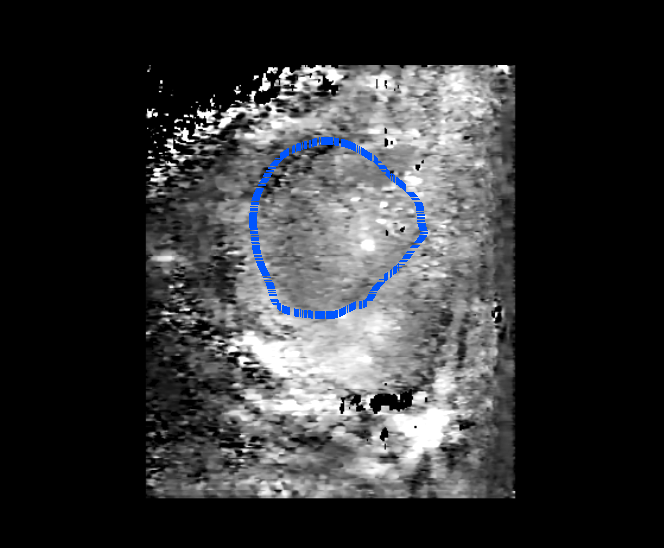
\includegraphics[width=0.3\textwidth]{tyler/sagittal_ARFI.png} &
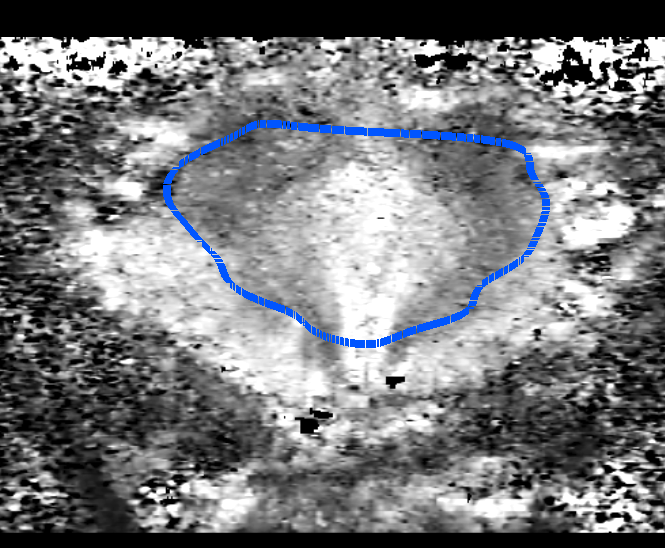
\includegraphics[width=0.3\textwidth]{tyler/coronal_ARFI.png} \\
Axial ARFI Outline & Sagittal ARFI Outline & Coronal ARFI Outline \\
\end{tabular}
\caption{Representative ultrasound prostate models from this study.  TOP ROWS:
    Prostate capsule 3D model (magenta) rendered from manual segmentation of
    the B-mode images, with the 3D model outlines superimposed on the central
    axial, sagittal and coronal B-mode images.  The primary segmentation plane
    was sagittal; however the axial and coronal planes were used to guide the
    segmentation to ensure 3D continuity of the capsule structure.  BOTTOM
    ROWS: Prostate central gland 3D model (blue) inside prostate capsule 3D model (magenta) rendered from manual
    segmentation of the ARFI images, with the prostate central gland 3D model outlines superimposed on
    the central axial, sagittal and coronal ARFI images.  The coronal ARFI
    imaging plane was the primary orientation used for image segmentation, but
    like capsule segmentation, the orthogonal planes were used to ensure continuity of
    the central gland in all three dimensions.}
\label{fig:arfi_segs} 
\end{figure}
